% !TEX root = ../modelo-ifg.tex

\chapter{Metodologia}
\label{cap:metodologia}

Este capítulo apresenta a abordagem metodológica empregada no desenvolvimento e na validação do
sistema de monitoramento remoto, caracterizada como uma pesquisa experimental aplicada. A execução
do trabalho foi estruturada em seis etapas fundamentais: (I) especificação e aprimoramento do
modelo de inteligência artificial; (II) definição e configuração do \textit{hardware} para
\textit{Edge AI}; (III) elaboração do projeto elétrico e de alimentação do sistema; (IV)
estabelecimento do meio de comunicação de dados em áreas remotas; (V) montagem do protótipo em
campo para testes de validação; e (VI) desenvolvimento de uma aplicação web de monitoramento,
controle e recebimento de alertas. Conforme ilustrado no fluxo da Figura~\ref{fig:fluxo_etapas},
cada uma dessas etapas desdobra-se em procedimentos específicos que asseguram o rigor e a
reprodutibilidade da pesquisa.

\begin{figure}[htbp]
  \centering
  \caption{Fluxo das etapas metodológicas do sistema de monitoramento.}
  \label{fig:fluxo_etapas}
  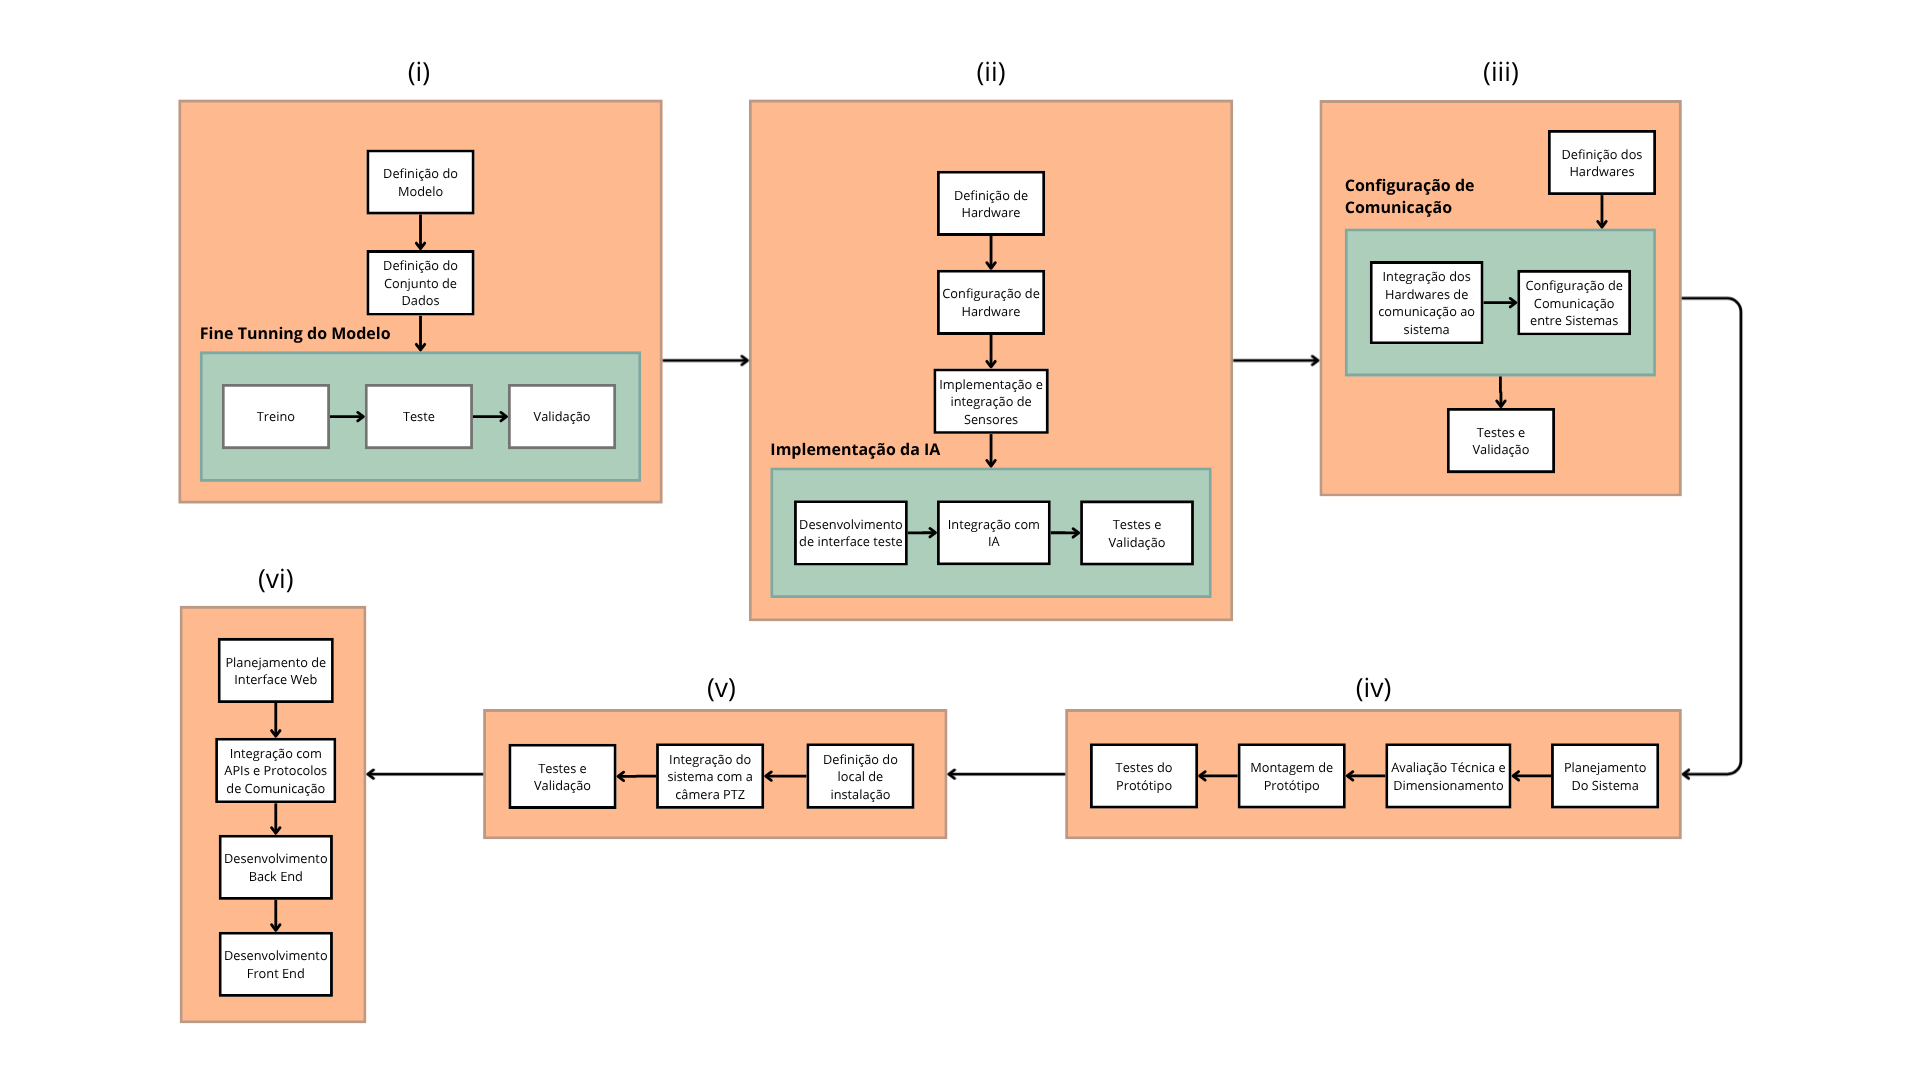
\includegraphics[width=\textwidth]{fig/fluxo-metodologia}
  \fontefig{Fonte: Autoral.}
\end{figure}

% ============================================================
\section{Etapa I -- Especificação e Aprimoramento do Modelo}
\label{sec:etapa_i}
% ============================================================

A seguinte etapa é composta por três processos: Definição do Modelo; Definição do Conjunto de
Dados; e \textit{Fine Tuning} do modelo que se divide em três subprocessos denominados Treino,
Teste e Validação. Esse conjunto de tarefas contribuem para a construção de um modelo de CNN capaz
de identificar focos de incêndio com um certo nível de eficácia determinado por um conjunto de
métricas a serem avaliadas.

\subsection{Definição do Modelo}
\label{subsec:def_modelo}

Analisando as diferentes arquiteturas existentes apresentadas na fundamentação teórica e os
modelos disponíveis no mercado, a variante intermediária da família YOLO26 \cite{jocher2026ultralytics}
estabelece um equilíbrio estratégico entre capacidade representacional e custo computacional,
viabilizando inferências em tempo real sem sobrecarregar os recursos limitados da plataforma de
borda. Essa superioridade na fronteira de eficiência é respaldada pelos resultados comparativos
apresentados na Figura~\ref{fig:yolo26_tradeoff}, na qual a família YOLO26 supera as gerações
anteriores na relação de compromisso entre acurácia média ($\overline{\text{AP}}$) e latência de
inferência em precisão de meia precisão (FP16).

\begin{figure}[htbp]
  \centering
  \caption{Curva de eficiência (\textit{trade-off} acurácia versus latência) comparando as
  variantes da família YOLO26 com arquiteturas anteriores de detecção de objetos no
  \textit{benchmark} COCO.}
  \label{fig:yolo26_tradeoff}
  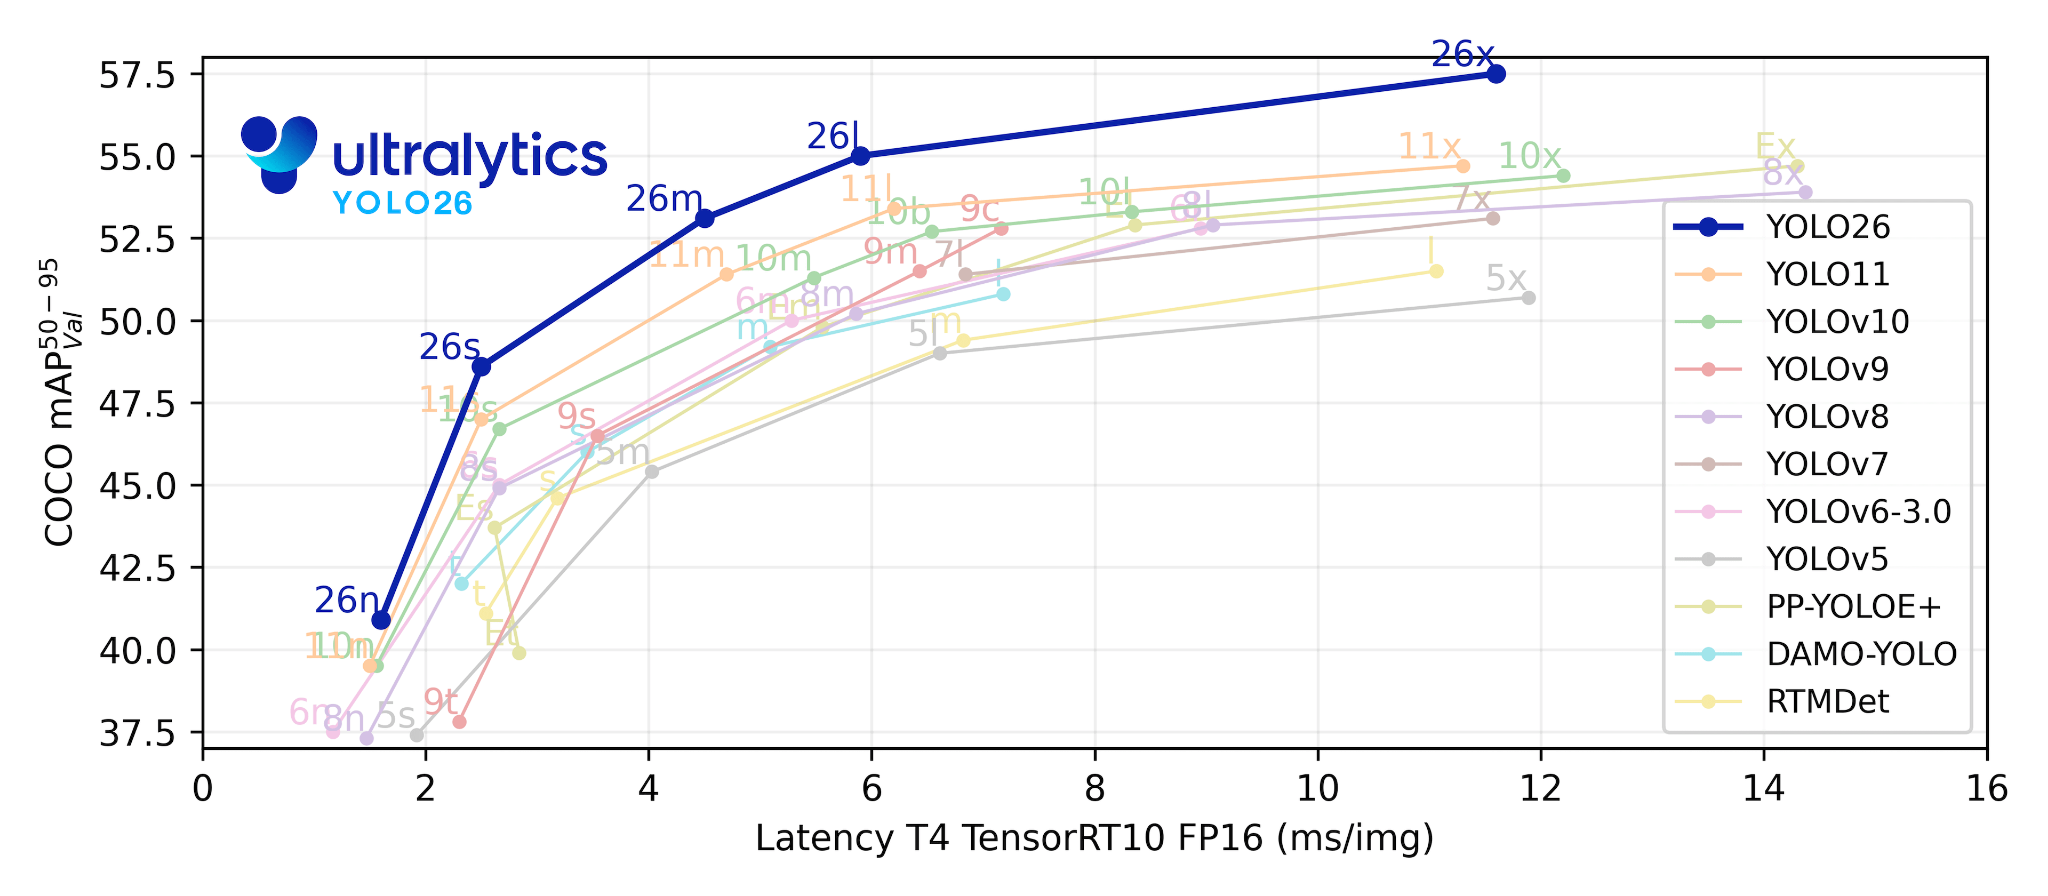
\includegraphics[width=0.85\textwidth]{fig/yolo26-tradeoff}
  \fontefig{Fonte: \citeonline{jocher2026ultralytics}.}
\end{figure}

Especificamente, a variante YOLO26m sendo executada pelo dispositivo NVIDIA Tesla T4 GPU, alcança
aproximadamente 53,1\% de mAP sob um tempo de execução de apenas 4,5\,ms por imagem e atingindo
até 194,4 GFLOPs, superando o desempenho de detecção de modelos de maior porte de gerações legadas
(como YOLOv5x e YOLOv7) enquanto preserva margem temporal e computacional suficiente para
processamento contínuo em nós embarcados.

As métricas apresentadas estão relacionadas ao \textit{dataset} COCO \cite{lin2014coco}, que
possui 80 classes diferentes em imagens anotadas, servindo como \textit{benchmark} para a avaliação
de modelos de detecção de objetos e segmentação de instâncias. Para o escopo deste trabalho, o
modelo foi delimitado à detecção de duas classes de interesse: fogo e fumaça. Essa especificação
busca não apenas identificar incêndios em estágios avançados de propagação, mas também viabilizar
a detecção precoce por meio da identificação de fumaça em fases iniciais. Além disso, a restrição
do vocabulário a essas duas classes visa otimizar a capacidade de generalização do modelo e
aumentar a precisão na extração de características específicas para esses alvos.

Em relação aos diferenciais arquitetônicos do modelo, a principal inovação reside na adoção de um
paradigma de treinamento com cabeçote duplo (\textit{dual-head architecture}), que combina uma
ramificação um-para-muitos (\textit{one-to-many}) rica em supervisão semântica durante a fase de
treino com uma ramificação um-para-um (\textit{one-to-one}) voltada ao descarte do
pós-processamento por Supressão de Não-Máximos (\textit{Non-Maximum Suppression} -- NMS) na etapa
de \textit{deployment}. No \textit{backbone} e \textit{neck}, a rede substitui estruturas
anteriores por blocos C3k2 otimizados e módulos de atenção espacial e de escala (S2A/PSA), aliando
a extração eficiente de características à redução de operações redundantes. Adicionalmente, o
treinamento emprega o otimizador MuSGD, uma combinação do algoritmo Muon para a atualização de
matrizes de peso bidimensionais com o SGD convencional, o que estabiliza o aprendizado profundo e
melhora a eficiência de convergência do modelo.

Com o intuito de adaptar essa arquitetura pré-treinada às especificidades do problema abordado, o
modelo é submetido a um processo de ajuste fino (\textit{fine-tuning}), cujos parâmetros,
hiperparâmetros e procedimentos experimentais são detalhados em outra seção do capítulo.

\subsection{Definição do \textit{Dataset}}
\label{subsec:def_dataset}

Conforme a metodologia apresentada no relatório de \citeonline{silva2026sistema}, que descreve todo
o processo de desenvolvimento do modelo de VC de detecção de foco de incêndio, o \textit{dataset}
do presente estudo foi constituído pelas imagens de \textit{Forest Fire, Smoke and Non-Fire Image
Dataset} \cite{minha2023forest}, referido como FFSNDataset. A base é composta, em seu conjunto de
treinamento, por 10.800 imagens positivas para fogo, 10.800 imagens positivas para fumaça e
10.800 imagens negativas apresentando uma distribuição equitativa das amostras no conjunto de
treino, porém não anotadas.

\subsection{\textit{Fine Tuning}}
\label{subsec:fine_tuning}

Diante o pré-processamento do modelo YOLO26m utilizando o \textit{dataset} COCO, será aplicado um
ajuste fino (\textit{fine tuning}) utilizando o \textit{dataset} indicado anteriormente com, no
total, 23.495 imagens, sendo 7.325 anotadas manualmente com o auxílio da plataforma
\textit{Computer Vision Annotation Tool} (CVAT) distribuídas pelo \textit{split} 70:20:10. Devido
a diversidade de cenários e tipos de incêndios dispostos nas imagens do FFSNDataset, que são
relevantes para aplicação dessa detecção no bioma do Cerrado, favoreceu a generalização do modelo.

De acordo com \citeonline{silva2026sistema}, o treinamento e a validação do modelo foi conduzido
na estação de trabalho Dell Precision Tower 5810, equipada com processador Intel Xeon E5-1650 v3
(6 núcleos físicos e 12 processadores lógicos), placa gráfica NVIDIA RTX A4500 e 128\,GB de
memória RAM DDR4, operando sob o sistema Microsoft Windows 11 Pro. Esse \textit{hardware} fornece
um ambiente estável para a execução de algoritmos de VC baseados na arquitetura YOLO. Os valores
dos hiperparâmetros empregados no treinamento são apresentados na Tabela~\ref{tab:hiperparametros}.

\begin{table}[htbp]
  \centering
  \caption{Hiperparâmetros utilizados para treinamento do modelo YOLO26m.}
  \label{tab:hiperparametros}
  \begin{tabular}{lr}
    \hline
    \rowcolor{gray!20}
    \textbf{Parâmetro} & \textbf{Valor} \\
    \hline
    Épocas (\texttt{epochs}) & 500 \\
    Resolução (\texttt{imgsz}) & 640 \\
    Paciência (\texttt{patience}) & 15 \\
    \texttt{lr0} & 0,01 \\
    \texttt{lrf} & 0,01 \\
    \texttt{momentum} & 0,937 \\
    \texttt{weight\_decay} & 0,0005 \\
    \texttt{warmup\_epochs} & 3,0 \\
    \texttt{warmup\_momentum} & 0,8 \\
    \hline
  \end{tabular}
  \begin{center}
    \fontetab{\citeonline{silva2026sistema}}
  \end{center}
  
\end{table}

Para avaliar o desempenho do modelo, utilizam-se métricas consolidadas na literatura para tarefas
de detecção de objetos: Precisão (P), Revogação (R), Pontuação F1 ($F1S$) e a Precisão Média
($AP$), calculadas a partir da classificação feita de Verdadeiros Positivos (VP), Falsos Positivos
(FP), Verdadeiros Negativos (VN), Falsos Negativos (FN) e a Intersecção Sob União (IoU).

A Precisão (P), apresentada pela equação~\eqref{eq:precisao}, mensura a proporção de detecções
corretas em relação ao total de predições realizadas pelo modelo:

\begin{equation}
  P = \frac{VP}{VP + FP}
  \label{eq:precisao}
\end{equation}

A Revogação (R), calculada pela equação~\eqref{eq:revogacao}, mensura a capacidade do algoritmo
em identificar corretamente todos os alvos reais presentes nas imagens, calculada pela razão entre
os acertos e o total de objetos reais:

\begin{equation}
  R = \frac{VP}{VP + FN}
  \label{eq:revogacao}
\end{equation}

Como costuma haver um \textit{trade-off} entre essas duas métricas, o $F1S$ é utilizado como a
média harmônica entre Precisão e Revogação, fornecendo uma medida única e balanceada do desempenho
global:

\begin{equation}
  F1S = 2 \cdot \frac{P \cdot R}{P + R}
  \label{eq:f1score}
\end{equation}

A validação espacial e categórica das predições do modelo é quantificada por meio da Interseção
sobre União (IoU), expressa pela Equação~\eqref{eq:iou}:

\begin{equation}
  IoU = \frac{|\hat{B} \cap B_{gt}|}{|\hat{B} \cup B_{gt}|}
  \label{eq:iou}
\end{equation}

em que $\hat{B}$ representa a caixa delimitadora (\textit{bounding box}) predita pelo modelo e
$B_{gt}$ denota a caixa delimitadora real (\textit{ground truth}). A detecção é considerada um VP
se o valor de IoU for maior ou igual a um limiar pré-definido $\tau_{IoU}$.

Para abrandar o impacto de oscilações na curva de Precisão versus Revogação (P-R),
calcula-se a Precisão Interpolada $p_{interp}(r)$ para um dado nível de revogação $r$, conforme
a Equação~\eqref{eq:prec_interp}:

\begin{equation}
  p_{interp}(r) = \max_{\tilde{r} \geq r} p(\tilde{r})
  \label{eq:prec_interp}
\end{equation}

na qual $p(\tilde{r})$ é a precisão medida no nível de revogação $\tilde{r}$. A partir dessa
interpolação, obtém-se a Precisão Média ($AP$) para uma classe $c$ sob o limiar $\tau$, que
corresponde à área sob a curva P-R, calculada pela Equação~\eqref{eq:ap}:

\begin{equation}
  AP_{c,\tau} = \int_{0}^{1} p_{interp}(r)\, dr
  \label{eq:ap}
\end{equation}

Por fim, a métrica global $mAP$ mensura a média das precisões médias ($AP$) integradas ao longo de
todas as $C$ classes e de um conjunto de limiares $T$, como formalizado na
Equação~\eqref{eq:map}:

\begin{equation}
  mAP_{50-95} = \frac{1}{C} \sum_{c=1}^{C} \left( \frac{1}{10} \sum_{t \in T} AP_{c,t} \right)
  \label{eq:map}
\end{equation}

% ============================================================
\section{Etapa II -- Definição e Configuração do Hardware de \textit{Edge AI}}
\label{sec:etapa_ii}
% ============================================================

Esta etapa metodológica detalha a seleção, o dimensionamento e a configuração da plataforma de
\textit{Edge AI}, cuja finalidade é executar a inferência do modelo YOLO26m. A seguir,
apresentam-se as especificações da arquitetura de hardware adotada, as ferramentas de compilação e
os procedimentos de otimização aplicados para viabilizar a detecção eficiente e de baixo consumo
energético em cenários de monitoramento de campo.

\subsection{Definição do Hardware}
\label{subsec:def_hardware}

A partir da contextualização feita no referencial teórico, o potencial do kit de desenvolvimento
\textit{NVIDIA Jetson Orin Nano} (8\,GB) como o núcleo de processamento do sistema
\cite{nvidia2026jetson}, que pode ser observado na Figura~\ref{fig:jetson_orin_nano}, é
selecionado como dispositivo \textit{Edge AI} para o processamento do modelo YOLO26m.

\begin{figure}[htbp]
  \centering
  \caption{Kit de Desenvolvimento Nvidia Jetson Orin Nano.}
  \label{fig:jetson_orin_nano}
  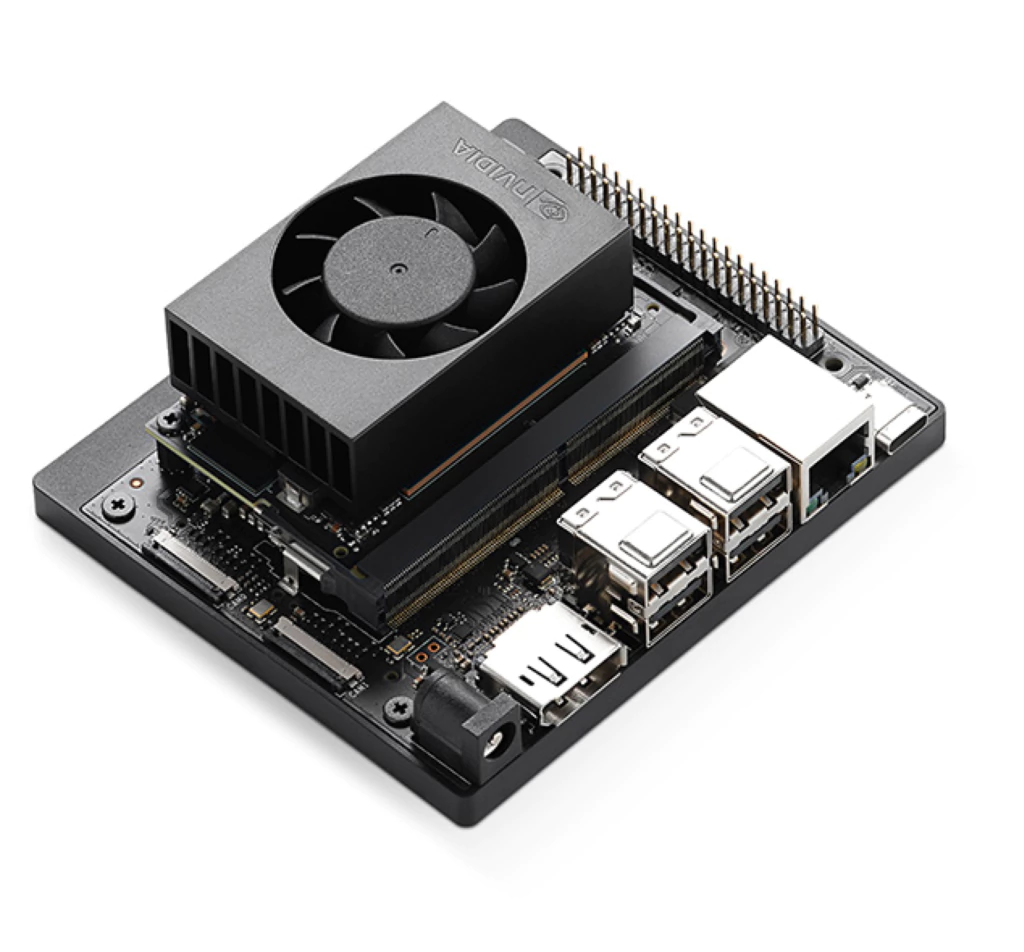
\includegraphics[width=0.60\textwidth]{fig/jetson-orin-nano}
  \begin{center}
    \fontefig{Adaptado de \citeonline{nvidia2026jetson}}    
  \end{center}

\end{figure}

O dispositivo apresenta um equilíbrio entre custo de aquisição, eficiência energética e capacidade
de aceleração para algoritmos densos de visão computacional em borda. Equipado com uma GPU baseada
na arquitetura NVIDIA Ampere dotada de 1.024 núcleos CUDA e 32 núcleos tensores
(\textit{Tensor Cores}), associada a uma CPU ARM Cortex-A78AE de 6 núcleos de 64 bits, o módulo
entrega até 40\,TOPS de desempenho de inferência em IA sob uma faixa de consumo térmico
configurável de apenas 7\,W a 15\,W. Complementarmente, a placa-base (\textit{carrier board}) do
kit oferece interfaces essenciais para a integração dos nós em campo, incluindo barramentos M.2
Key~M (PCIe Gen4~$\times$4) para a instalação de unidades de armazenamento velozes em SSD NVMe,
conector Gigabit Ethernet nativo para recepção direta do fluxo de vídeo da câmera via rede e
conectividade serial para interfaceamento de comunicação externa \cite{nvidia2026jetson}. Essa
densidade computacional permite executar modelos convolucionais modernos em tempo real diretamente
na torre, mantendo a autonomia necessária para operação sustentada por bancos de baterias e painéis
fotovoltaicos sem comprometer a acurácia de detecção em campo.

\subsection{Configuração de Hardware}
\label{subsec:config_hardware}

Visando superar as limitações de largura de banda e durabilidade associadas aos cartões microSD
convencionais, a estação embarcada foi configurada com um disco de estado sólido NVMe SSD M.2 de
256\,GB, dedicado tanto ao armazenamento do sistema operacional quanto à hospedagem do ambiente de
execução e dos modelos pré-treinados. O processo de preparação da plataforma iniciou-se com a
gravação da imagem oficial do \textit{JetPack~6.x} (baseado no Ubuntu~22.04~LTS) no SSD NVMe por
meio da ferramenta \textit{NVIDIA SDK Manager}, garantindo o particionamento direto no disco de
alta velocidade e a configuração dos \textit{bootloaders} do sistema. Em seguida, foram instalados
e vinculados os drivers proprietários da arquitetura Ampere, as bibliotecas do CUDA \textit{Toolkit}
(versão~12.2), o cuDNN para aceleração de operações convolucionais e o TensorRT, assegurando a
pilha de \textit{software} necessária para a compilação e execução eficiente das inferências do
modelo de detecção na ponta.

\subsection{Integração da IA}
\label{subsec:integracao_ia}

A arquitetura de software desenvolvida para a plataforma Nvidia Jetson Orin Nano foi concebida de
forma modular, articulando a execução da inferência de aprendizagem profunda a serviços de
comunicação e transmissão de dados em tempo real. A detecção de objetos na ponta é gerenciada pelo
\textit{framework} Ultralytics, encarregado do carregamento e da execução otimizada dos pesos do
modelo YOLO26m ajustado e armazenado em arquivo \textit{checkpoint} do PyTorch, que é o
\textit{framework} base da Ultralytics.

A camada de disponibilização de dados é estruturada sobre um servidor
\textit{web micro-framework} Flask, que expõe a interface de monitoramento e os
\textit{endpoints} de transmissão de vídeo. Para viabilizar o acesso remoto seguro ao fluxo do
servidor sem a necessidade de IPs públicos fixos no ambiente de campo, utiliza-se a ferramenta
Pyngrok, criando um túnel HTTP/HTTPS dinâmico sobre a porta local. O sistema de alertas e
notificação imediata é gerenciado pela API do Twilio (via módulo \textit{sending}), encarregada do
envio automático de mensagens de emergência ao identificar focos de incêndio. Por fim, a gestão de
chaves de API, senhas e parâmetros de rede é tratada pelo Python-Dotenv, isolando as variáveis de
ambiente sigilosas do código-fonte principal e assegurando as boas práticas de segurança do sistema.

A aceleração computacional na plataforma Nvidia Jetson Orin Nano é viabilizada por sua GPU
integrada baseada na arquitetura Ampere, composta por 1.024 núcleos CUDA e 32 Tensor Cores
dedicados. No contexto de inferência de modelos de aprendizagem profunda como o YOLO26, a execução
na GPU é essencial para realizar o processamento massivamente paralelo de convoluções e operações
matriciais sobre os \textit{frames} de vídeo em tempo real. Uma característica estrutural dessa
plataforma é a Arquitetura de Memória Unificada (\textit{Unified Memory Architecture} -- UMA), na
qual a CPU e a GPU compartilham a mesma memória RAM física (8\,GB LPDDR5). Esse arranjo reduz
significativamente a latência do sistema, uma vez que elimina a necessidade de copiar tensores de
imagem entre a memória do sistema e a memória de vídeo dedicada ($V_{RAM}$) através de barramentos
PCI Express.

Para alocar e otimizar o uso da GPU durante a execução da IA, o ambiente de \textit{software} é
configurado por meio da pilha de bibliotecas da Nvidia (\textit{JetPack}). A comunicação direta
com o hardware ocorre via \textit{driver} proprietário e CUDA Toolkit, enquanto operações
convolucionais complexas são aceleradas pela biblioteca cuDNN. Na camada de aplicação, o modelo é
otimizado via TensorRT, que recompila o grafo da rede neuronal, aplicando técnicas de fusão de
camadas, eliminação de operações mortas e quantização de precisão (conversão de ponto flutuante de
32 bits, $FP32$, para precisão reduzida de 16 bits, $FP16$, ou inteiros de 8 bits, $INT8$). Essa
otimização permite que as rotinas do \textit{framework} Ultralytics operem diretamente sobre o
dispositivo \texttt{cuda:0}.

Visando assegurar o rendimento máximo da GPU sem restrições térmicas ou limitação de potência
(\textit{thermal throttling}), a configuração do sistema embarcado inclui o ajuste dos perfis de
desempenho do sistema operacional. Por meio do utilitário \texttt{nvpmodel}, a placa é definida
para o modo de operação de maior consumo e capacidade computacional (MAXN ou 15\,W), desativando
os perfis de economia de energia. Adicionalmente, executa-se o \textit{script}
\texttt{jetson\_clocks}, que fixa as frequências de clock da GPU, da CPU e dos barramentos de
memória em seus valores nominais máximos, garantindo a estabilidade da taxa de FPS e a
previsibilidade temporal durante a inferência na ponta.

% ============================================================
\section{Etapa III -- Estabelecimento dos Meios de Comunicação}
\label{sec:etapa_iii}
% ============================================================

% Seção a ser desenvolvida em revisão futura.

% ============================================================
\section{Etapa IV -- Elaboração do Projeto Elétrico}
\label{sec:etapa_iv}
% ============================================================

O projeto elétrico do sistema foi elaborado com base nas diretrizes técnicas de
\citeonline{pinho2014manual} e em conformidade com as normas brasileiras \cite{abnt2019nbr16690} e
\cite{abnt2004nbr5410}. Embora o dispositivo de \textit{Edge AI} do sistema tenha sido definido,
o dimensionamento e a seleção dos equipamentos da fonte de alimentação demandam identificação
precisa e caracterização elétrica de todos os dispositivos que compõem a carga do sistema. Esta
etapa é direcionada ao planejamento da integração do protótipo para posteriormente realizar a
montagem.

\subsection{Seleção de Equipamentos}
\label{subsec:selecao_equipamentos}

Para completar o sistema de monitoramento de focos de incêndio, além do dispositivo de borda e dos
equipamentos que compõem a alimentação do sistema, deverá ser constituído de uma câmera dedicada
que possua algumas das tecnologias identificadas na fundamentação teórica, um módulo de Internet
4G e um modem de internet para realizar o compartilhamento de rede.

Em relação ao dispositivo de câmera que será utilizado, com o propósito de assegurar a relação
custo-benefício da solução desenvolvida, selecionou-se um equipamento de captura capaz de operar
tanto no espectro visível quanto na faixa NIR em curtas distâncias operacionais. O sistema
prioriza a detecção de incêndios durante o período diurno e em condições meteorológicas favoráveis,
contornando a necessidade imediata de sensores térmicos de elevado custo financeiro.

A partir dessas premissas de viabilidade econômica e robustez de sensoriamento, é analisada a
viabilidade da câmera PTZ \textit{Intelbras VIP 5432 SD IR IA FT} \cite{intelbras2025vip5432}. O
dispositivo apresenta uma relação custo-benefício estratégica para o projeto ao dispensar matrizes
térmicas de alto custo, entregando resolução de 4 megapixels (2560\,$\times$\,1440) a 30 quadros
por segundo aliada a um conjunto óptico varifocal com zoom óptico motorizado de 32$\times$
(distância focal de 4,8\,mm a 154\,mm). Essa configuração óptica viabiliza a varredura panorâmica
contínua em 360° (\textit{pan}) associada à aproximação detalhada de alvos a longas distâncias,
atendendo aos requisitos de cobertura territorial de grandes extensões de preservação ambiental.
Para operar sob condições de baixa luminosidade e transição noturna, a câmera conta com sensor
CMOS de alta sensibilidade com tecnologia \textit{Starlight} e um sistema de iluminação ativa no
espectro infravermelho próximo (NIR) composto por LEDs com alcance efetivo de até 150\,metros
\cite{intelbras2025vip5432}. Por fim, o equipamento dispõe de carcaça metálica com grau de
proteção IP67 e antivandalismo IK10, garantindo a integridade física do nó de captura contra
intempéries climáticas severas, como chuvas torrenciais, poeira e variações bruscas de temperatura
comuns ao ambiente de campo.

\begin{figure}[htbp]
  \centering
  \caption{Câmera PTZ Intelbras VIP 5432 SD IR IA FT.}
  \label{fig:camera_intelbras}
  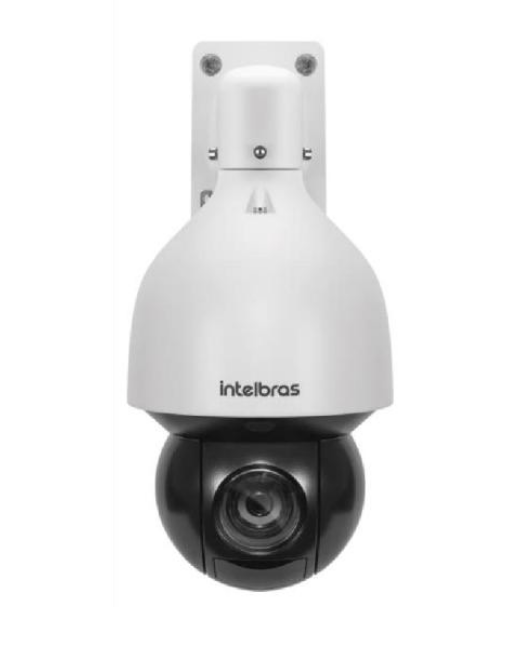
\includegraphics[width=0.50\textwidth]{fig/camera-intelbras-vip5432}
  \begin{center}
    \fontefig{\citeonline{intelbras2025vip5432}}
  \end{center}
\end{figure}

\subsection{Projeto Elétrico}
\label{subsec:projeto_eletrico}

% Seção a ser desenvolvida em revisão futura.

\subsection{Dimensionamento}
\label{subsec:dimensionamento}

% Seção a ser desenvolvida em revisão futura.

% ============================================================
\section{Etapa V -- Montagem do Protótipo em Campo}
\label{sec:etapa_v}
% ============================================================

% Seção a ser desenvolvida em revisão futura.

% ============================================================
\section{Etapa VI -- Desenvolvimento da Interface Web}
\label{sec:etapa_vi}
% ============================================================

% Seção a ser desenvolvida em revisão futura.
